\documentclass{sig-alternate}
%\usepackage[latin1]{inputenc} % Windows
\usepackage[utf8x]{inputenc} % Linux (unicode package needed)
% \usepackage[applemac]{inputenc} % Mac


\usepackage{url}


\usepackage{balance}


\usepackage{graphicx}
\usepackage{caption}
\usepackage{subcaption}
\usepackage{hyperref}




\usepackage{xcolor}
\usepackage{color}


\definecolor{editorGray}{rgb}{0.95, 0.95, 0.95}
\definecolor{editorOcher}{rgb}{1, 0.5, 0} % #FF7F00 -> rgb(239, 169, 0)
\definecolor{editorGreen}{rgb}{0, 0.5, 0} % #007C00 -> rgb(0, 124, 0)


\usepackage{upquote}
\usepackage{listings}
\lstdefinelanguage{JavaScript}{
  morekeywords={typeof, new, true, false, catch, function, return, null, catch, switch, var, if, in, while, do, else, case, break},
  morecomment=[s]{/*}{*/},
  morecomment=[l]//,
  morestring=[b]",
  morestring=[b]'
}


\lstdefinelanguage{HTML5}{
        language=html,
        sensitive=true, 
        alsoletter={<>=-},
        otherkeywords={
        % HTML tags
        <html>, <head>, <title>, </title>, <meta, />, </head>, <body>,
        <canvas, \/canvas>, <script>, </script>, </body>, </html>, <!, html>, <style>, </style>, ><
        },  
        ndkeywords={
        % General
        =,
        % HTML attributes
        charset=, id=, width=, height=,
        % CSS properties
        border:, transform:, -moz-transform:, transition-duration:, transition-property:, transition-timing-function:
        },  
        morecomment=[s]{<!--}{-->},
        tag=[s]
}


\lstset{%
    % Basic design
    backgroundcolor=\color{white},
    basicstyle={\small\ttfamily},   
    frame=l,
    % Line numbers
    xleftmargin={0.75cm},
    numbers=left,
    stepnumber=1,
    firstnumber=1,
    numberfirstline=true,
    % Code design   
    keywordstyle=\color{blue}\bfseries,
    commentstyle=\color{darkgray}\ttfamily,
    ndkeywordstyle=\color{editorGreen}\bfseries,
    stringstyle=\color{editorOcher},
    % Code
    language=HTML5,
    alsolanguage=JavaScript,
    alsodigit={.:;},
    tabsize=2,
    showtabs=false,
    showspaces=false,
    showstringspaces=false,
    extendedchars=true,
    breaklines=true,        
    % Support for German umlauts
    literate=%
    {Ö}{{\"O}}1
    {Ä}{{\"A}}1
    {Ü}{{\"U}}1
    {ß}{{\ss}}1
    {ü}{{\"u}}1
    {ä}{{\"a}}1
    {ö}{{\"o}}1
}


\colorlet{punct}{red!60!black}
\definecolor{background}{HTML}{FEFEFE}
\definecolor{delim}{RGB}{20,105,176}
\colorlet{numb}{magenta!60!black}


\lstdefinelanguage{json}{
    basicstyle=\small\ttfamily,
    % numbers=left,
    % numberstyle=\scriptsize,
    % stepnumber=1,
    % numbersep=8pt,
    % showstringspaces=false,
    % breaklines=true,
    % frame=lines,
    backgroundcolor=\color{background},
    literate=
     *{0}{{{\color{numb}0}}}{1}
      {1}{{{\color{numb}1}}}{1}
      {2}{{{\color{numb}2}}}{1}
      {3}{{{\color{numb}3}}}{1}
      {4}{{{\color{numb}4}}}{1}
      {5}{{{\color{numb}5}}}{1}
      {6}{{{\color{numb}6}}}{1}
      {7}{{{\color{numb}7}}}{1}
      {8}{{{\color{numb}8}}}{1}
      {9}{{{\color{numb}9}}}{1}
      {:}{{{\color{punct}{:}}}}{1}
      {,}{{{\color{punct}{,}}}}{1}
      {\{}{{{\color{delim}{\{}}}}{1}
      {\}}{{{\color{delim}{\}}}}}{1}
      {[}{{{\color{delim}{[}}}}{1}
      {]}{{{\color{delim}{]}}}}{1},
}


\begin{document}










\title{x-project: a novel approach to design document-oriented Web Applications based on HTML5 Web Components}


\numberofauthors{4} 
\author{
\alignauthor
Andrea D'Amelio\\
  \affaddr{Universit\`a Roma Tre}\\
  \affaddr{Dipartimento di Ingegneria}\\
  \affaddr{Universit\`a Roma Tre}\\
  \affaddr{Rome, Italy}\\
  \email{damelio@dia.uniroma3.it}
\alignauthor
Enrico Marino\\
  \affaddr{Universit\`a Roma Tre}\\
  \affaddr{Dipartimento di Ingegneria}\\
  \affaddr{Universit\`a Roma Tre}\\
  \affaddr{Rome, Italy}\\
  \email{marino@dia.uniroma3.it}
\and
\alignauthor
Tiziano Sperati\\
  \affaddr{Universit\`a Roma Tre}\\
  \affaddr{Dipartimento di Ingegneria}\\
  \affaddr{Universit\`a Roma Tre}\\
  \affaddr{Rome, Italy}\\
  \email{sperati@dia.uniroma3.it}
\alignauthor
Federico Spini\\
  \affaddr{Universit\`a Roma Tre}\\
  \affaddr{Dipartimento di Ingegneria}\\
  \affaddr{Universit\`a Roma Tre}\\
  \affaddr{Rome, Italy}\\
  \email{spini@dia.uniroma3.it}
}





\maketitle
\begin{abstract}
Lorem ipsum dolor sit amet, consectetur adipisicing elit, sed do eiusmod
tempor incididunt ut labore et dolore magna aliqua. Ut enim ad minim veniam,
quis nostrud exercitation ullamco laboris nisi ut aliquip ex ea commodo
consequat. Duis aute irure dolor in reprehenderit in voluptate velit esse
cillum dolore eu fugiat nulla pariatur. Excepteur sint occaecat cupidatat non
proident, sunt in culpa qui officia deserunt mollit anim id est laborum.


\end{abstract}


\category{H.4}{Information Systems Applications}{Miscellaneous}
\category{D.2.8}{Software Engineering}{Metrics}[complexity measures, performance measures]
\terms{Theory}
\keywords{Web Application, Web Platform, Single Page Application, Content Management System, Web Components, API}









\section{Introduction}
A web application framework is a software framework that is designed to support the development of dynamic web applications.
To speed up web application development, action based frameworks mostly rely on external configuration files
Regarding to numerous open source web frameworks, it becomes so difficult for developers to select a suitable framework for web applications development. Because of that, the purpose of this paper is to help web developers to easier choose the right framework for development of their web applications. The paper will analyze a few open source Java component based frameworks. Additionally, the paper will provide basic features of the analyzed frameworks as well as represent their most important characteristics. Also, in this paper the analyzed web frameworks will be compared and summarized [1, 2, 3].











\section{State of the art}
Con Web Application intendiamo tutte le applicazioni distribuite sul web.
Questo tipo di applicazioni sono accessibili su diverse tipologie di rete, come ad esempio una architettura tipica di tipo client-server.
Le prime web apps consistevano infatti nella generazione di pagine standard HTML/XHTML; successivamente con l'evolversi delle tecnologie associate e soprattutto con la nascita di nuovi standard, si cominciarono a distribuire attraverso di essa documenti in formato ancora più semplici, come l'XML.
La parte dinamica lato client (o client-side) di questi sistemi informatici è affidata sempre a linguaggi standard, come ad esempio JavaScript, che sono inclusi in tutti i browser. Il crescente successo conseguito da librerie esperte, ormai veri e propri framework come JQuery, tecnologie dinamiche come AJAX, oppure plug-in, come il conosciuto Flash Player, consente oggi di pilotare ed arricchire le interfacce utente in modo completo ed efficiente.
Il Web Application Framework è un software di supporto per lo sviluppo di web site e web application. Lo scopo principale di questo software è quello di aiutare il lavoro associato al web introducendo delle librerie per effettuare diverse operazioni come l’accesso a basi di dati o la creazione di template HTML.
{http://it.wikipedia.org/wiki/Applicazione_web}











\subsection{CMS platforms}
One generally accepted definition of Content Management System is: ``A system that lets you apply management principles to content''[4].




It is simple to elicit an evolutionary path in the history of management system whose milestones are identifiable in \emph{Joomla!}\cite{joomla}, \emph{Wordpress}\cite{wordpress} and \emph{KeystoneJS}\cite{keystone}.


Alongside these milestones entire constellations of analogous experiences popped up, but we considered them not relevant since they borrowed main features and constitutive approaches from cited ones. 


Starting from \emph{Joomla!}, a framework that drove in the engineering into the world of web content management. Joomla! powers more than 2,7% of the largest 1,000,000 web sites in the world. [504] Anyway, nowadays, Joomla! results unwieldy and, due to its monolithic approach, not complied to current web features.




\emph{Wordpress}, instead is used by more than 23.3\% of the top 10 million websites (as of January 2015) [6]. Wordpress develop CMS’s idea, driving in the intention to use CMSs to build Web Application. Wordpress, with its plugin, aims to limber user experience. The availability of more than 37,000 plugins, because it lets to create sites to non-experts too.
Anyway, further customizations, other than the ones introduced by plugins, are difficult to deploy due to loosely code engeneering of this tool.


Finally, \emph{KeystoneJs} stand in the last position. Minimal and agile, KeystoneJS, embody the new era of the CMS, letting the user to make his own personal web application.


In the spite of focusing on very minimal features, a Mention goes to Ghost \cite{ghost}[300], a non-profit, open source blogging Node.js based platform, which represents a transversal experience although minimal brings SOMETHING IN,.


Eventually, X-Project, for the reasons the will be clear in the remaining of this paper, could be thought as the last standing in this path of decreasing monolithic approach and increasing customization and code engineering.

















\section{X-Project}
x-project is a set of libraries and API-centric HTML5 Web Components based Web Application and CMS framework.















\subsection{Philosophy}
''Everything is an element'', even an AJAX request. Every part of the website is encapsulated inside an element. Even functional components such as HTTP services (AJAX calls), pages and routing logic are encapsulated inside elements. We push Web Components' philosophy beyond all limits so that users can reach a very high level of customization and ease of use.




Component-based Software Engineering denotes the process of building software by (re)using pre-built software components. The main benefit of component-based software is the``time-to-marke'' \cite{4773208}, thus reducing the cost of developing the software. A software component is a unit of composition with contractually specified interfaces and explicit context dependencies. 
Additionally, a component is a software element that conforms to a component model and can be independently deployed and composed \cite{cite:test} [13]. Component based software is developed interconnecting building blocks, therefore, a high degree of reusability and modularity is achieved by this type of applications [14]. 















\subsection{Architecture}
To design a Client-server API-centric architecture for Single Page Application the project has been based on some cutting edge enabling technologies.
X-Project architectural stack is based on the following technologies.


Client-side is entirely based on Web Components.
Web Components are a collection of standards which are working their way through the W3C and landing in browsers at the moment. In a nutshell, they allow us to bundle markup and styles into custom HTML elements. [11]
 \emph{Custom Elements}\cite{customel}, \emph{HTML Imports}\cite{customel}, \emph{Templates}\cite{customel}, \emph{Shadow DOM}\cite{customel}.


Considering that Web Components is a work-in-progress standard, not all modern browsers support all the Web Components functions.
To avoid this problem has been developed Webcomponents.js, a set of polyfills built on top of the Web Components specifications. It makes it possible for developers to use these standards today across all modern browsers.[304, 305]


In the last year there were multiple frameworks built on top of Web Components, but only Polymer-Project, by Google, has established itself. 
Polymer makes it easier and faster to create elements, from a button to a complete application across desktop, mobile, and beyond. 
The Polymer core provides a thin layer of API on top of web components. 
It expresses Polymer's opinion, provides the extra sugaring that all Polymer elements use, and is meant to help make developing web components much easier [103].
It provides several powerful features that streamline element creation such as: custom events and delegation, mixins, accessors and component lifecycle functions.


In addition to framework, there are three major libraries: Iron-Elements, Component Kitchen and CustomElements.io. The first, in the previous version called Paper-Elements, is developed by Google, as a support of the Polymer-Project. At the moment it counts about twenty-five elements in addition to other thirty Paper-Elements.[306]
However, at the moment, the most complete library is, no doubt, CustomElements.io: an open source user-contributed library that counts more than a thousend elements. [307]








Looking at the server-side, the most used Web Server Application frameworks are based on Node.js.
Node.js is a platform built on Chrome's JavaScript runtime for easily building fast, scalable network applications. 
As shown by Linkedin case, Node.js became, lately, a standard de facto [302].




One of Node.js based frameworks, maybe the best-known, is Express.js.
Express is a minimal and flexible Node.js web application framework that provides a set of features for web and mobile applications.[303]




Moreover, there is a framework, that works closely to Express.js named Strongloop - LoopBack.
Loopback is a set of Node.js modules to develop Web Servers applications.
An application interacts with data sources through the LoopBack model API, available locally within Node.js, remotely over REST. [10]




All these framework allow the client-server development with single page application approach. This particular development paradigm makes clearer the gap between server and client, rendering data on client side.
A single-page application, is a web application or web site that fits on a single web page with the goal of providing a more fluid user experience akin to a desktop application.












% \begin{figure}[!htbp]
% \centering
% 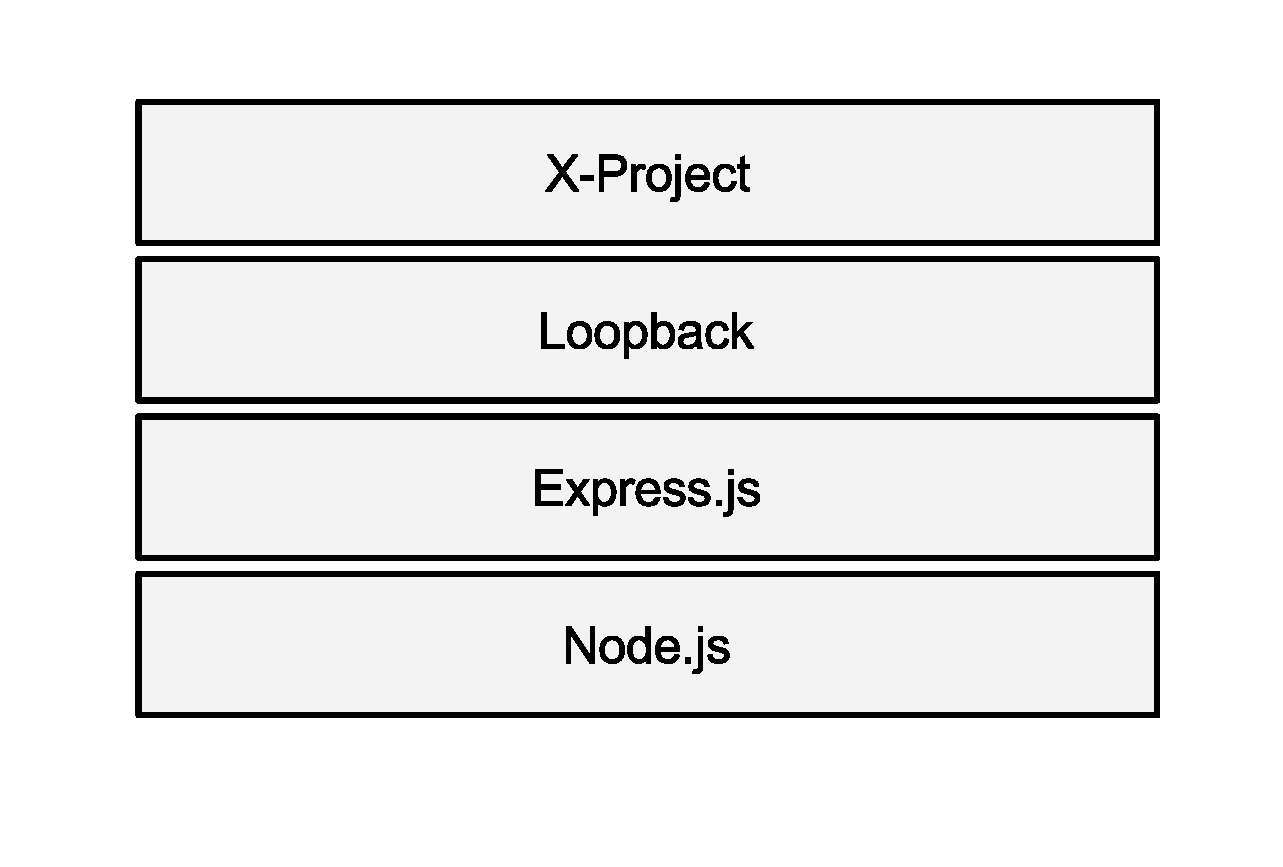
\epsfig{file=images/stack.eps, height=0.2\textwidth}
% \caption{Technology stack}
% \label{fig:tech-stack}
% \end{figure}


\begin{figure}[!h]
 \centering
 \begin{subfigure}[b]{0.53\linewidth}
 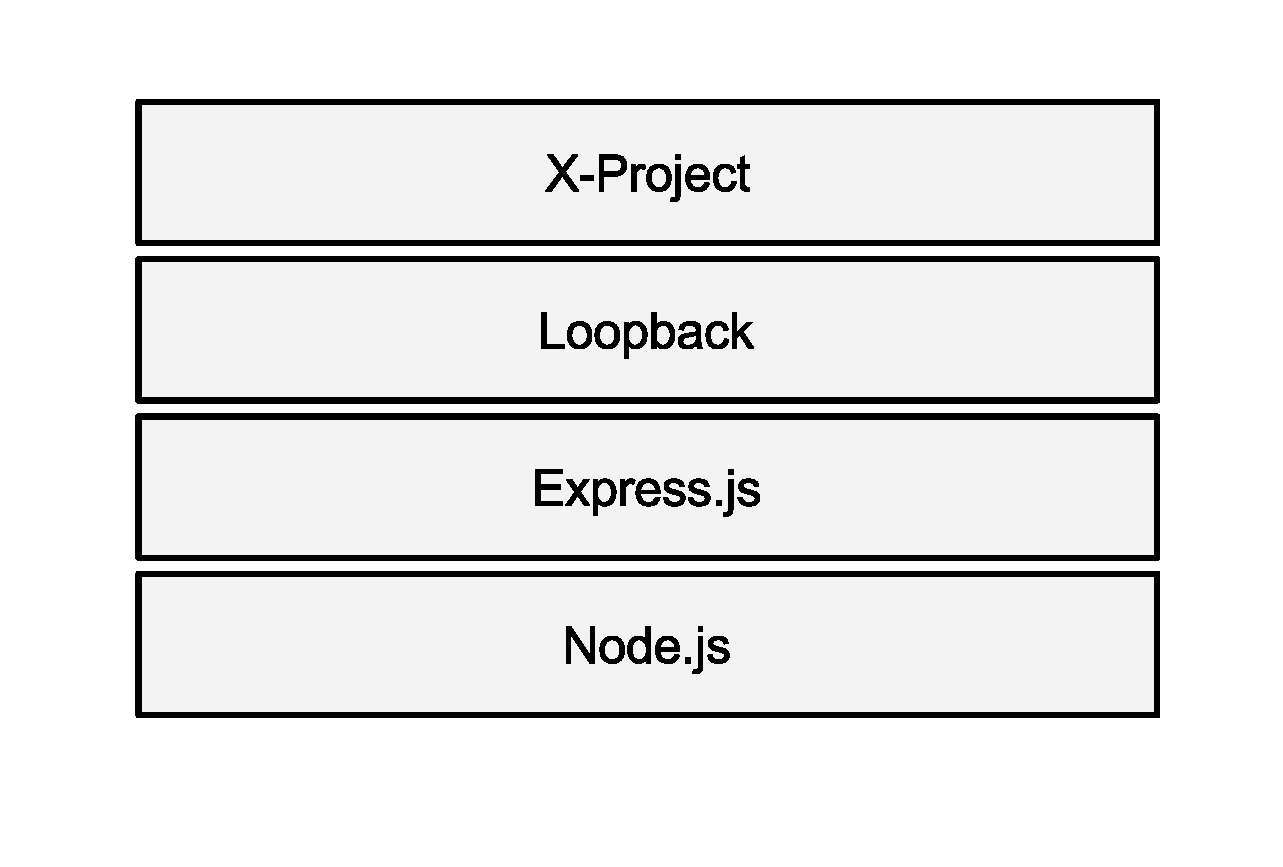
\includegraphics[width=\textwidth]{images/stack.eps} 
 \caption{Technology stack.}
 \label{fig:tech-stack}
 \end{subfigure}
 ~
 \begin{subfigure}[b]{0.43\linewidth}
 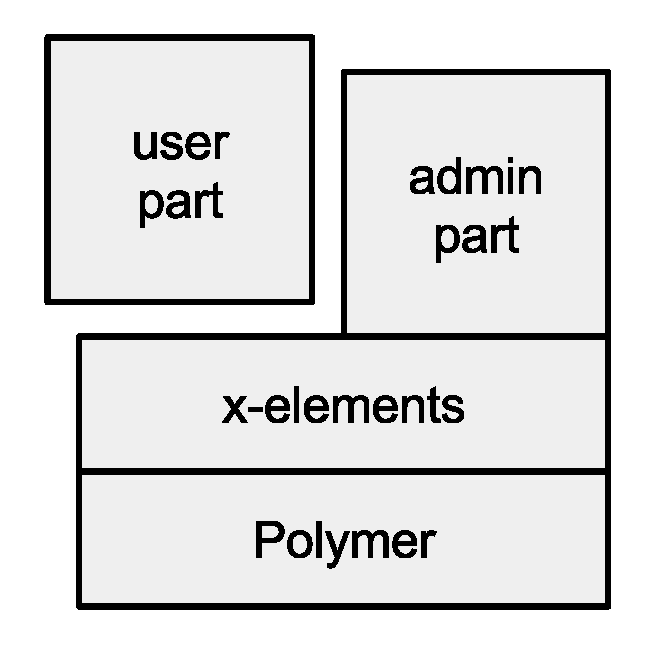
\includegraphics[width=\textwidth]{images/client-arch.eps}
 \caption{Client-side architecture}
 \label{fig:client-arch}
 \end{subfigure}
 
 % \caption{Office building: 
 % (a) the schematic plan; 
 % (b) the simplified 3D model generated for testing on the field 
 % the indoor mapping project described in this paper.
 % }
 % \label{fig:sogei}
\end{figure}


% \begin{figure}[!htbp]
% \centering
% 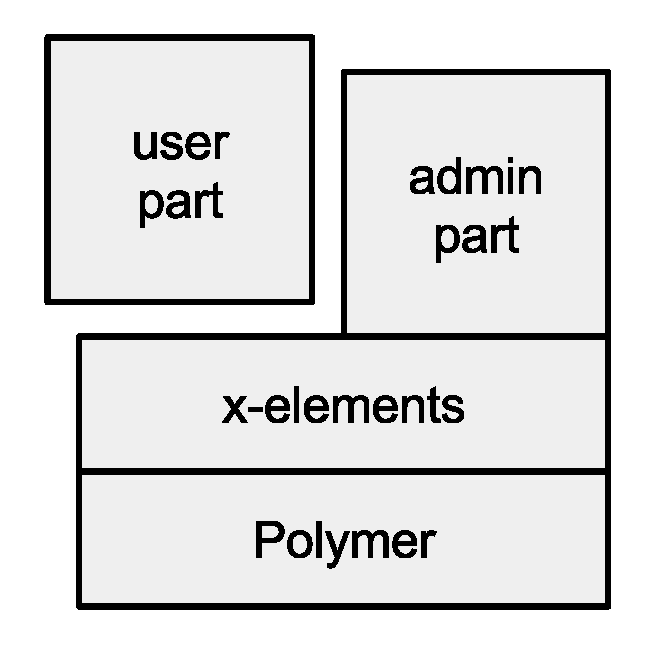
\epsfig{file=images/client-arch.eps, height=0.2\textwidth}
% \caption{Client-side architecture}
% \label{fig:client-arch}
% \end{figure}


  


 















\subsection{Server-side}
As said before, server-side architecture is based on Strongloop Loopback framework and Node.js. The Web Application development is mostly data-driven. Firstable it takes to be defined models: using JSON format, the developer can describe the entity schema.
Then, automatically, Loopback generates model’s APIs: CRUD operations are available by default and is possible to add new APIs. In order to extend the APIs, the developer can add remote functions to models or add hooks to existing APIs.
Moreover, the server doesn’t handle the session using cookies, but it does via tokens: every request needs a token signature.
Even the token system is handled during the model definition: in fact, an Access Control Layer (ACL) is provided. With this layer, developers can restrict access to certain APIs only to specific users.




To speed up web application development, action based frameworks mostly rely on external configuration files and less on Java code [15]
avviene tramite JSON




The platform design is document-oriented, so the minimum step required is to define the models of the application, defining correspondent .json documents.
x-project json document for model definition extends the loopback json document, adding a special property \$type, that is used to automatically generate the appropriate input form elements in the admin control panel. 













\subsubsection{third parties services}
As said in [20], an important feature of a CMS is media storage (documents, images and video). X-Project provides a remote storage service: it, thanks to adapters, is completely disjointed from the storage service chosen and it allows, unlike Loopback framework does, to store files directly from the client, not passing via server side.
For this reason, has been implemented a direct upload tool to AWS Amazon S3 storage service.




\begin{figure}[!htbp]
\centering
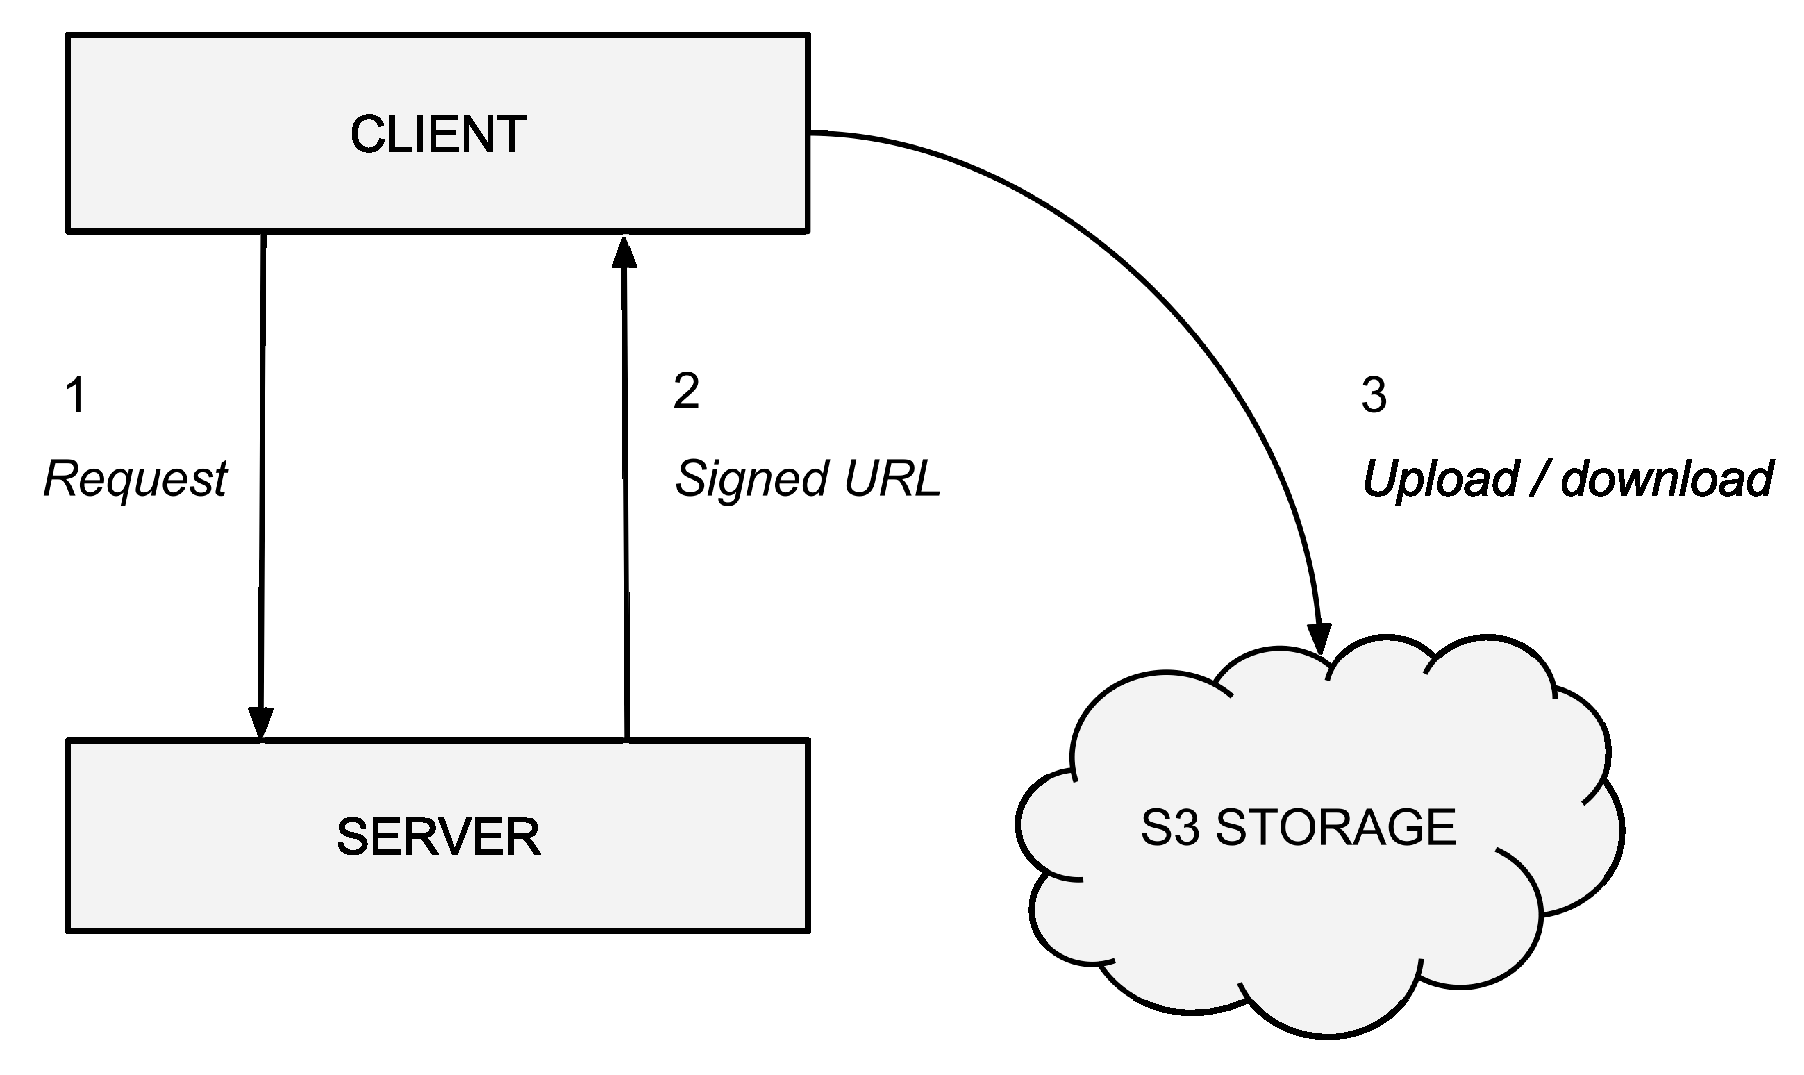
\epsfig{file=images/services.eps, height=0.24\textwidth}
\caption{Third parties services}
\label{fig:services}
\end{figure}




This tool uses signed request paradigm to authenticate files upload and download.
1. To achieve an upload, the client must launch an upload request to S3 Service. 
2. Then the request must be signed, with the private key, by the server, that returns the authenticated URL. 
3. At this moment, the client, can send the authenticated request to the server, that, after the verification, will validate the action.
In this process, the server and S3 Service share the private key, but the client doesn’t. So the system is secure.




To use the direct upload module on S3, it needs only to create a public bucket on AWS and to set the keys in the node.js module.
On the client-side, there is a dedicate element, <x-input-element>, that communicates with the API that generates signed requests and that provides the upload service.




Download service follows the same pattern both to get the full list of files in the bucket and to get just a part of it. 







\subsection{Client-side}


Client-side can be divided in two parts: Admin part and User part.
Admin part is automatically generated from the model defined. It let the admin to manage (via CRUD operations) the models.
User part depends on the type of the Web Application that has been implemented.
It is the part the final user interact with.


% \begin{figure}[!htbp]
% \centering
% 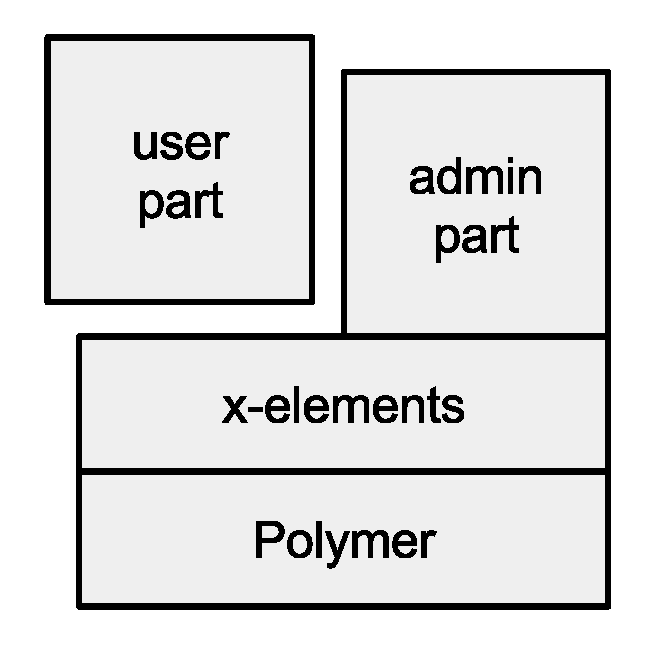
\epsfig{file=images/client-arch.eps, height=0.2\textwidth}
% \caption{Client-side architecture}
% \label{fig:client-arch}
% \end{figure}


Client-side pages design could rely on x-elements library, a set of Polymer element for local routing, API requests, forms, and style. 


Each data type of a model is associated with an input element.
These \$type and correspondent input elements are: \emph{number} $\rightarrow$ \texttt{<x-number>}, \emph{string} $\rightarrow$ \texttt{<x-input>}, \emph{select} $\rightarrow$ \texttt{<x-select>}, \emph{date} $\rightarrow$ \texttt{<x-date>}, \emph{enum} $\rightarrow$ \texttt{<x-radio>}, \emph{email} $\rightarrow$ \texttt{<x-email>}, \emph{textarea} $\rightarrow$ \texttt{<x-textarea>}, \emph{url} $\rightarrow$ \texttt{<x-url>}, \emph{boolean} $\rightarrow$ \texttt{<x-checkbox>}, \emph{money} $\rightarrow$ \texttt{<x-money>}, \emph{password} $\rightarrow$ \texttt{<x-password>}, \emph{file} $\rightarrow$ \texttt{<x-file>}.



















\subsubsection{Routing elements}
X-Project allows to design using single page application pattern: in order to have this opportunity, there are elements designed to handle client-side routing.


\begin{description}
\itemsep1pt\parskip0pt\parsep0pt
        \item[x-router] implements routing system using HTML5 Push State APIs. The route to page mapping is encapsulated into x-route elements, in fact x-router contains an x-route element for each route desired. Moreover, if the route matched by the router is parametrized, it will pass parameters as attributes of the element.
        \item[x-route] represents a single route to a page inside the application. This element has two major attributes: route and page. 
\item[x-link], is an anchor element ({\tt <a>}) extension designed to prevent default behavior of requiring pages to the server and manage the routing locally. \end{description}


\begin{lstlisting}[language=HTML5, label={lst:add-a-label-here}, captionpos=b,  caption=Add a caption here.]
<x-router>
  <x-route 
    route="admin/collections/:name/:id/edit" 
    page="page-model-edit"></route>
         <!-- others x-route -->
</x-router>
\end{lstlisting}







\subsubsection{Page models list}


\begin{lstlisting}[language=HTML5, label={lst:add-a-label-here}, captionpos=b,  caption=Add a caption here.]
<a is="app-link" 
  href="admin/collections/Posts">
  Posts</a>
\end{lstlisting}


\begin{lstlisting}[language=HTML5, label={lst:add-a-label-here-n2}, captionpos=b,  caption=model list page.]
<page-collection>
  <api-collection-get 
    name="{{collection_name}} 
    filter="{{filter}}"
    collection="{{collection}}">
  </api-collection-get>
  <part-collection-filter 
    name="{{collection_name}}"  
    filter="{{filter}}">
  </part-collection-filter>
  <part-list 
    list="{{collection}}">
  </part-list>
  <part-paginator 
    list="{{list}}" 
    filter="{{filter}}"
    current="{{page}}">
  </part-paginator>
</page-collection>
\end{lstlisting}



\subsubsection{Page edit model}
\begin{lstlisting}[language=HTML5, label={lst:add-a-label-here}, captionpos=b,  caption=Add a caption here.]
<a is="app-link" 
  href="admin/collections/Posts/1/edit">
  edit post</a>
\end{lstlisting}


\begin{lstlisting}[language=HTML5, label={lst:add-a-label-here-n2}, captionpos=b,  caption=model edit page.]
<page-model-edit>
  <api-model-get 
    name="{{collection_name}}" 
    model-id="{{model_id}}"
    model="{{model}}">
  </api-get-model>
  <part-form-edit 
    model="{{model}}" 
    schema="{{schema}}">
  </part-form-edit>
</page-model-edit>
\end{lstlisting}


\begin{lstlisting}[language=HTML5, label={lst:add-a-label-here-n2}, captionpos=b,  caption=model edit form.]
<part-form-edit>
  <template is="dom-repeat" 
    item="{{model.properties}}>
    <input-x property="{{item}}">
    </input-x>
  </template>
</part-form-edit>
\end{lstlisting}







\subsubsection{API elements}
x-elements provide a set of elements to handle model API
(questo inglese è pessimo, potremmo aggiungere “and thing" ogni tanto…) 


\begin{description}
\itemsep1pt\parskip0pt\parsep0pt
       \item[api-(get|post)-collection] to retrieve a collection or create a model
       \item[api-(get|put|delete)-model] to retrieve/update/delete a model
\end{description}




These api-call wrapper handle filters and pagination.


\begin{lstlisting}[language=HTML5, label={lst:add-a-label-here}, captionpos=b,  caption=Add a caption here.]
<api-get-collection 
  name="Posts" perpage="10" page="2" filter="{{filter}}"
  collection="{{posts}} count="{{count}}"></api-get-collection>
\end{lstlisting}


this element perform an HTTP GET request to “/api/Posts" using filter and returning the first 10 items of the second page and the number of items retrieved (for pagination purpose).
filter attribute is an object that is added in querystring
that has the following filters:











\subsubsection{Form elements}
X-Elements provides a basic set of input elements used to automatically generate the admin panel. Anyway these elements can be used by the developer to design pages generally.


Native input types are: x-input, x-textarea, x-number, x-date, x-datetime are respectively elements designed to short text, long text, numbers, date, date and time. x-location, based on Google Place APIs, allows to choose locations using autocomplete add-on. x-file used to file remote storage, based on the direct upload module, described in[paragrafo server-side/third-party-services].







\subsubsection{Style elements}
x-project style is based on iron-flex-layout a CSS library component  [501][https://github.com/PolymerElements/iron-flex-layout]
 based on the CSS Flexible Box Layout Module [503] [http://www.w3.org/TR/css3-flexbox/] using CSS variables [http://dev.w3.org/csswg/css-variables/] and CSS mixins [502][http://oocss.org/spec/css-mixins.html] 





\section{Case study}
In this section we design a blog platform. 


\subsection{server-side}
For a blog platform the models are: Author, Post and Tag.


\begin{lstlisting}[language=json, label={lst:add-a-label-here-n3}, captionpos=b, caption=Post model.]
{
  "name": "Post",
  "properties": {
    "title": { "$type": "string" },
    "posted": { "$type": "date" },
    "content": { "$type": "text" },
  }, 
  "relations": [{ 
    "name": "author", 
    "type": "belongs_to",
    "model": "Author",
  }, {
    "name": "tags", 
    "type": "has_many",
    "model": "Tag",
  }]
}
\end{lstlisting}



























\subsection{client-side}
The admin part is just generated by x-project, 
so it remains to define the page to list the posts and to read one post.


\begin{lstlisting}[language=HTML5, label={lst:add-a-label-here-n4}, captionpos=b,  caption=Add a caption here.]
<x-route>
  <x-route route="posts" page="page-posts"></x-route>
  <x-route route="posts/:post_id" page="page-post"></x-route>
</x-route>
\end{lstlisting}


\begin{lstlisting}[language=HTML5, label={lst:add-a-label-here-n4}, captionpos=b,  caption=Add a caption here.]
<page-posts>
  <api-get-collection name="Posts" page="{{page}}" perpage="10"
    collection="{{collection}}" count="{{count}}"></api-get-collection>
  <part-posts-list list="{{collection}}"></part-posts-list>
  <part-pages count="{{count}}" perpage="10" current="{{page}}"></part-pages>
</page-posts>
\end{lstlisting}


\begin{lstlisting}[language=HTML5, label={lst:add-a-label-here-n4}, captionpos=b,  caption=Add a caption here.]
<page-post>
  <api-get-model name="Posts" model-id="{{post_it}}"
    model="{{post}}"></api-get-model>
  <h1>{{post.title}}</h1>
  <h2>by <span>{{post.author}}</span></h2>
  <h3>{{post.date}}</h3>
  <p>{{post.content}}</p>
</page-post>
\end{lstlisting}



















\section{Conclusion}
conclusions











\subsection{Microservices}


Microservices















\subsection{Benchmarking}
In the present time open source content management system (CMS) has gained a big market. Lots of varieties are available based on functionality and platform.
As told, there are different performance criteria like page load time (PLT), page size (PS), number of request, number of CSS and JS files etc. while comparing all these parameters we could come to conclusion that which CMS should be used under what conditions [19].




Generally all CMSs fulfill common task of content like create, edit, publish. But above mention CMS are providing good user support, security, more plug-ins, documentation etc than other.
 
As shown in [20] there are about thirty features to analyze to make a comparison of CMSs. We can design six important classes of features that summarize all the features.


Admin Management, Data Management, User Management, UI Management, Web Content Management, Multimedia Data Management.















\bibliographystyle{abbrv}
\bibliography{x-project-paper}
\end{document}
